%% Revised IEEE conference paper prepared from the saved evidence package.
%% Numerical claims are restricted to results already present in the package;
%% no unrun experiment or unsupported sensitivity analysis is reported.
\documentclass[conference]{IEEEtran}
\usepackage{cite}
\usepackage{amsmath,amssymb}
\usepackage{graphicx}
\graphicspath{{ieee/}{}}
\usepackage{booktabs}
\usepackage{url}

\hyphenation{epi-demi-o-log-i-cal}

\begin{document}

\title{Anchoring is What Matters: SEIR-Informed Graph Forecasting for Dengue}

\author{\IEEEauthorblockN{Tharusha Perera, Praveen De Silva, Janith Mahanama,
Bimsara Udurawana, \\
Maleesha Kumarasinghe, Praveen Nawarathna}
\IEEEauthorblockA{Department of Computer Science and Engineering, University of Moratuwa\\
Moratuwa, Sri Lanka\\
\{tharushap.23, praveend.23, janithm.23, bimsarau.23,\\
kumarasinghemp.23, praveenn.23\}@cse.mrt.ac.lk}}

\maketitle

\begin{abstract}
Graph neural networks can learn spatial dependence between districts, but they do not explicitly encode the infection-stage dynamics that constrain epidemic trajectories.
We study a hybrid forecaster that couples an adaptive graph encoder to a susceptible--exposed--infectious--recovered (SEIR) decoder, with population-and-susceptibility anchoring and a learned gate to persistence.
The model is evaluated three weeks ahead on a reconstructed series of 559 weekly reports from 25 Sri Lankan districts. % EV-216, EV-007
Reconstruction exposed a formula error in a published source table; on the earlier benchmark array, excluding the six forecast windows that touch that week reduces persistence RMSE from 44.80 to 29.52 cases per district-week. % EV-220
Across nine rolling origins, the proposed configuration has the lowest point-estimate RMSE among 30 learned configurations, 27.45 versus 28.54 for persistence, a 3.8\% relative reduction (paired difference -1.10; 95\% interval -2.84 to 0.65). % EV-200, EV-215
Within the same GCN encoder, replacing a free SEIR rate with the population-and-susceptibility anchored rate reduces RMSE from 28.43 to 27.62. % EV-210, EV-213
However, the proposed model is not statistically distinguishable from persistence after Holm adjustment, and the current experiments do not isolate the SEIR equations from the effects of anchoring and gating. % EV-219
The evidence therefore supports a competitive, mechanistically constrained graph forecaster and a data-quality contribution, but not a confirmed forecasting advantage over persistence.
\end{abstract}

\begin{IEEEkeywords}
dengue forecasting, epidemic modeling, graph neural networks, persistence baseline, mechanistic learning, SEIR model
\end{IEEEkeywords}

\section{Introduction}
Dengue causes recurring epidemics in Sri Lanka~\cite{tissera2020severe}.
Short-horizon district forecasts can support planning for clinical capacity and vector-control activity.
Spatio-temporal graph models are attractive because districts are not independent: neighbouring areas can share mobility, environmental conditions, and reporting patterns~\cite{weng2024graph}.
Their learned dynamics, however, need not respect the latent exposed and infectious stages that constrain how incidence can evolve.

For a one- to three-week forecast, recent reported counts may therefore be informative but incomplete: some infections that shape the near future are not yet represented as reported cases.
Compartmental models provide a way to encode this structure.
An SEIR model tracks movement through susceptible, exposed, infectious, and recovered states, and Liu et al.~\cite{liu2025seirlstm} showed that a neural model can learn the force of infection for Sri Lankan dengue.
We ask a narrower question: can an SEIR-informed decoder be integrated with a graph forecaster in a way that is competitive with both graph-only prediction and a strong persistence baseline?
Persistence is essential here because weekly dengue counts change gradually over short horizons, and the earlier Sri Lankan graph benchmark does not report it~\cite{weng2024graph}.

This study makes three contributions.
First, we construct a hybrid graph--SEIR forecaster whose transmission rate is anchored to district population and susceptible fraction and whose output can fall back to persistence through a learned gate.
Second, we rebuild and source-check the district surveillance series and show that one spreadsheet error materially changes the apparent difficulty of the legacy benchmark.
Third, we evaluate 30 learned configurations against persistence over nine rolling origins, reporting paired uncertainty and ablations that distinguish free versus anchored rates, bare versus gated SEIR heads, and alternative graph encoders.
Because the protocol and model family evolved during development, we interpret these results as development evidence rather than independent confirmation.

\section{Related Work}
Weng et al.~\cite{weng2024graph} adapted several graph encoders to Sri Lankan dengue forecasting, including STGAT, A3T-GCN, ASTGCN, DCRNN, and AAGCN~\cite{huang2019stgat,bai2021a3tgcn,guo2019astgcn,li2018dcrnn,shi2019aagcn}.
DengueGNN also studies graph-based dengue prediction~\cite{gulmohamed2026denguegnn}, while Graph WaveNet introduced the learned-adjacency construction used in our adaptive encoder~\cite{wu2019graphwavenet}.
In parallel, Liu et al.~\cite{liu2025seirlstm} combine neural prediction with a human SEIR model for dengue in Sri Lanka.
EINNs and CausalGNN incorporate epidemiological assumptions into neural forecasters, and MepoGNN couples graph learning with metapopulation epidemic dynamics~\cite{rodriguez2023einns,wang2022causalgnn,cao2023mepognn}.
Prior work therefore provides graph forecasting and epidemiologically informed neural modeling separately; our study tests their combination against persistence on the same source-checked district series and examines which constraints within the SEIR head matter.

\section{Data}\label{sec:data}
\subsection{Case-series reconstruction}
The reconstructed series contains 559 weekly reports for 25 districts from June 15, 2013, to February 24, 2024; seven reports are missing and are left missing. % EV-216
Any forecast window whose inputs or targets touch a missing report is excluded.
Each forecasting sample maps the previous three weeks of district counts to the next three weeks. % EV-007
The earlier benchmark array, referred to here as the legacy array, contains 459 rows without a verified calendar. % EV-002

\begin{figure}[t]
\centering
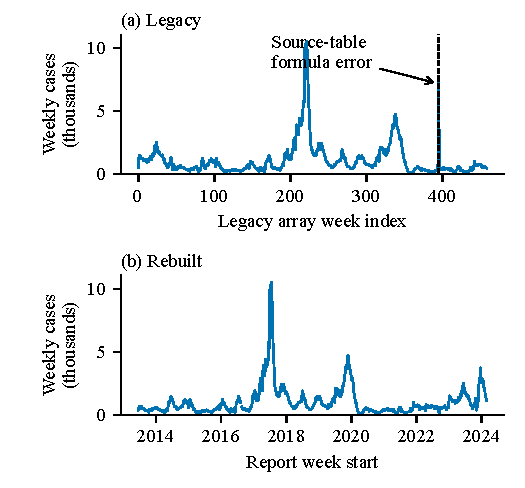
\includegraphics[width=\columnwidth]{figures/fig_data.pdf}
\caption{National weekly cases summed over 25 districts. (a) Legacy benchmark array, with the source-table formula error marked. (b) Reconstructed series used for the main evaluation; gaps denote missing reports.}
\label{fig:data}
\end{figure}

During reconstruction, each district row was checked against the printed national total.
Legacy row 395 corresponds to the report for December 26, 2020, to January 1, 2021~\cite{epid2021wer0248}. % EV-222
In its weekly row, 15 of 24 inner cells equal the sum of the two preceding cells; the district entries sum to 7165 while the printed weekly national total is 35. % EV-222
The same report's year-to-date row, which equals the first-week count at the start of a year, is consistent with its printed total of 351 when Kalmunai is included. % EV-222
We therefore treat the legacy spike as a spreadsheet formula error rather than an outbreak and use the year-to-date row when reconstructing that report.

\subsection{Spatial graph}
Districts are graph nodes and shared borders define the intended static adjacency.
Checking the border list against GADM polygons gives 57 shared borders, 114 directed entries, and 139 entries after self-loops. % EV-221
The saved development experiments used the benchmark graph, which contains two additional one-directional entries, Kandy--Ampara and Kegalle--Kalutara, that are not shared borders, for 141 entries in total. % EV-221
We retain those historical scores for traceability and treat this graph mismatch as a limitation rather than silently replacing the graph without rerunning the models.

\section{SEIR-Informed Graph Network}\label{sec:methods}
Fig.~\ref{fig:arch} summarizes the model.
The graph encoder captures inter-district dependence, while the decoder constrains within-district trajectories through daily compartment flows.
For each district and forecast horizon, the encoder produces a read-out $r$ that is mapped either directly to a forecast or to parameters of the SEIR head.

\begin{figure*}[t]
\centering
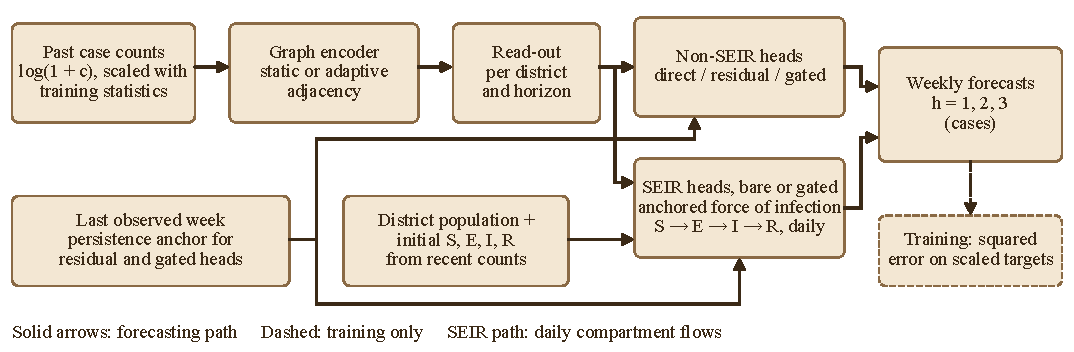
\includegraphics[width=\textwidth]{figures/fig_arch.pdf}
\caption{SEIR-informed graph network. The graph encoder and read-out feed either a non-SEIR head or an SEIR head that converts a learned force of infection into weekly incidence through daily compartment flows. Residual and gated heads use the last observed week as a persistence anchor.}
\label{fig:arch}
\end{figure*}

\subsection{Encoder and prediction heads}
Counts $c_{i,t}$ for district $i$ and week $t$ are transformed using training-period statistics,
\begin{equation}
z_{i,t}=\{\log(1+c_{i,t})-\mu\}/\sigma.
\label{eq:z}
\end{equation}
The persistence anchor $p$ repeats the standardized latest count at all three horizons.
The GCN encoder projects the input to 64 dimensions and applies two residual graph layers, $H'=H+\mathrm{Dropout}(\mathrm{ReLU}(AHW+b))$, where $A$ is the row-normalized adjacency with self-loops. % EV-177
The adaptive encoder learns $A_{\rm ad}=\mathrm{softmax}(\mathrm{ReLU}(E_1E_2^\top))$ from standard-normal $25\times10$ node embeddings shared by both layers and excluded from weight decay. % EV-177

We compare non-mechanistic heads that test three different departures from persistence.
A direct head outputs $r$; a residual head outputs $p+r$; and a gated head learns how far to move from persistence, $p+g(r-p)$, with $g=\mathrm{sigmoid}(a)$ and $a$ initialized at $-2$. % EV-178
The bare SEIR head outputs the standardized simulator count $z(\hat c)$, while the gated SEIR head outputs $p+g\{z(\hat c)-p\}$.
All learned models minimize squared error on the standardized log scale.
This stabilizes highly skewed counts, but the objective is not perfectly aligned with count-scale RMSE; we therefore treat count-scale RMSE as an evaluation metric rather than as the quantity directly optimized.

\subsection{SEIR decoder}
For each horizon, the decoder advances susceptible, exposed, infectious, and recovered fractions one day at a time,
\begin{equation}
\begin{aligned}
f_S&=S(1-e^{-\lambda\Delta t}),\quad f_E=E(1-e^{-\omega\Delta t}),\\
f_I&=I(1-e^{-\gamma\Delta t}),\quad
\hat c_{i,h}=\rho_{\rm eff}N_i\sum_{d=1}^{7} f_E^{(d)}.
\end{aligned}
\label{eq:seir}
\end{equation}
Flows are computed from the current state and moved along $S\rightarrow E\rightarrow I\rightarrow R$; predicted weekly cases are the daily exposed-to-infectious flows summed over seven days and scaled by district population $N_i$ and an effective reporting fraction.
We use $\omega=0.7/7=0.1$ and $\gamma=1/7$ per day, corresponding to mean exposed and infectious periods of ten and seven days, following Liu et al.~\cite{liu2025seirlstm}. % EV-011
The base reporting fraction is $\rho=1/11$, with a learned global multiplier $\rho_{\rm eff}=\rho\exp(q)$. % EV-011, EV-217
Initial infectious and exposed fractions are derived from $c_{t-1}/(\rho N_i)$ and $c_{t-2}/(\rho N_i)$ and clipped to $[10^{-6},0.5]$. % EV-170
The susceptible fraction is $\mathrm{clip}(0.318-C_{<t}/(\rho N_i),0.01,1)$, where $C_{<t}$ is the cumulative earlier report count. % EV-170
The value 0.318 is one minus the 68.2\% seroprevalence measured in suburban Colombo~\cite{jeewandara2015sero} and is applied to every district. % EV-170, EV-223
A multiplier $2\,\mathrm{sigmoid}(v)$ rescales the exposed fraction, either globally or per district from the encoder. % EV-217

The force of infection is either free or anchored.
The free rate exponentiates the read-out plus a learned bias.
The anchored rate supplies an epidemiological scale before the learned adjustment,
\begin{equation}
\lambda^*_{i,h}=\frac{\max(c_{i,t-1},0.5)}{7\rho_{\rm eff}N_iS_i}
\exp\{\mathrm{clip}(r_{i,h},-10,10)\}.
\label{eq:anchor}
\end{equation}
The leading factor is the daily rate that would reproduce last week's reported count under the current population, susceptible fraction, and reporting scale; the read-out therefore learns a multiplicative departure from that anchor.
Both free and anchored rates are multiplied by a learned spatial import term $\exp\{0.1\beta(u_i-\bar u)\}$, where $u_i=\log\max((AI)_i,10^{-9})$. % EV-217
A mass-action ablation instead uses a learned daily transmission coefficient times the infectious fraction, recomputed each day, without the import term.
We refer to the adaptive encoder with the gated anchored SEIR head and encoder-derived $E_0$ as the \emph{Adaptive SEIR-GNN}.

\section{Development Evaluation Protocol}\label{sec:setup}
\begin{figure}[t]
\centering
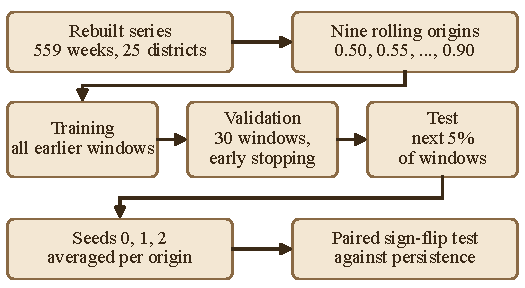
\includegraphics[width=\columnwidth]{figures/evaluation_protocol.pdf}
\caption{Development evaluation. At each of nine origins, models are trained on earlier windows, early-stopped on 30 validation windows, and scored on the next 5\% of forecast starts. Seed-averaged origin scores are paired with persistence.}
\label{fig:protocol}
\end{figure}

We use rolling-origin evaluation (Fig.~\ref{fig:protocol}) with nine cut-offs from 0.50 to 0.90 of the valid forecast-start list in steps of 0.05; each held-out block contains the next 5\% of starts. % EV-186
The 30 starts immediately before each cut-off form the validation set. % EV-182
This grid was selected after earlier development runs using a three-origin protocol and another nine-origin grid, so it should not be interpreted as a preregistered confirmatory test. % EV-227
Each learned configuration is trained with seeds 0, 1, and 2, giving 27 runs per configuration; persistence is deterministic. % EV-101

All learned models use Adam with learning rate 0.003 and weight decay 0.0001, batch size 32, cosine decay, gradient clipping at 5, at most 300 epochs, and early stopping on count-scale validation RMSE with patience 40. % EV-175, EV-224
Because every start predicts three weeks, the final training and first validation targets share two calendar weeks, and the final validation and first held-out targets do the same. % EV-218
Consequently, early stopping has access to outcomes that also occur in the first held-out windows; we report the design transparently and treat it as a limitation.

The evaluation contains 30 learned configurations plus persistence: GCN, LSTM, STGAT, A3T-GCN, ASTGCN, and AAGCN with direct, residual, free-rate gated-SEIR, and bare-SEIR heads, together with six adaptive/anchored variants. % EV-179
Seeds are averaged within origin before inference.
For each learned configuration, the paired unit is the nine origin-level RMSE differences from persistence.
We report count-scale RMSE and MAE, RMSE by horizon, a descriptive 95\% $t$ interval for the paired difference, and an exact two-sided sign-flip test with Holm adjustment across all 30 model-versus-persistence comparisons. % EV-200, EV-219
With nine origins, the smallest attainable Holm-adjusted $p$ is 0.117, limiting power for small effects. % EV-226

\section{Results}\label{sec:results}
\begin{table*}[t]
\centering
\caption{Development results on the rebuilt series (nine rolling origins, three seeds; benchmark graph, unpurged splits). These are not the prospective results of Table~\ref{tab:prospective}. RMSE and MAE are in cases per district-week, averaged over origins and seeds; horizon columns report RMSE. $\Delta$ is the seed-averaged paired RMSE difference from persistence with a 95\% t interval over origins (negative is better). Bold marks the lowest test RMSE (the proposed Adaptive SEIR-GNN); an interval that includes zero shows no clear difference from persistence.}
\label{tab:main}
\small\setlength{\tabcolsep}{3pt}
\begin{tabular}{@{}p{2.85in}rrrrrr@{}}
\toprule
Model & $h=1$ & $h=2$ & $h=3$ & RMSE & MAE & $\Delta$ [95\% CI] \\
\midrule
Persistence (last week) & 23.47 & 27.94 & 33.26 & 28.54 & 13.94 & -- \\ % EV-200

GCN, direct & 23.10 & 27.82 & 32.68 & 28.17 & 13.66 & -0.37 [-1.88, +1.14] \\ % EV-201

GCN, residual (baseline GNN) & 23.24 & 27.79 & 32.47 & 28.12 & 13.62 & -0.42 [-1.54, +0.70] \\ % EV-202

LSTM, direct & 23.65 & 28.22 & 33.38 & 28.73 & 14.00 & +0.19 [-1.99, +2.37] \\ % EV-203

ASTGCN, direct & 23.92 & 28.54 & 33.45 & 28.94 & 14.27 & +0.40 [-2.02, +2.81] \\ % EV-204

AAGCN, direct & 24.11 & 29.10 & 33.66 & 29.26 & 14.06 & +0.72 [-1.57, +3.00] \\ % EV-205

STGAT, direct & 42.60 & 44.55 & 46.75 & 44.71 & 22.17 & +16.17 [+4.24, +28.11] \\ % EV-206

ASTGCN, residual & 23.07 & 28.08 & 33.66 & 28.65 & 13.98 & +0.11 [-1.68, +1.90] \\ % EV-207

Adaptive GCN, residual & 23.07 & 27.78 & 32.15 & 27.94 & 13.61 & -0.60 [-1.81, +0.61] \\ % EV-208

GCN, SEIR, free rate & 27.58 & 40.81 & 50.14 & 40.77 & 17.97 & +12.23 [+2.67, +21.80] \\ % EV-209

GCN, gated SEIR, free rate & 22.86 & 28.04 & 33.29 & 28.43 & 13.51 & -0.11 [-3.23, +3.00] \\ % EV-210

Adaptive GCN, SEIR, anchored & 23.99 & 28.81 & 35.29 & 29.80 & 13.84 & +1.26 [-1.47, +3.98] \\ % EV-211

Adaptive GCN, gated SEIR, mass-action & 22.90 & 28.02 & 33.19 & 28.39 & 13.52 & -0.16 [-3.16, +2.85] \\ % EV-212

GCN, gated SEIR, anchored & 22.49 & 27.38 & 32.04 & 27.62 & 13.39 & -0.92 [-2.60, +0.76] \\ % EV-213

Adaptive GCN, gated SEIR, anchored & 22.51 & 27.09 & 31.85 & 27.45 & 13.31 & -1.09 [-2.81, +0.63] \\ % EV-214

\textbf{Adaptive GCN, gated SEIR, anchored, learned $E_0$} & \textbf{22.45} & \textbf{27.07} & \textbf{31.88} & \textbf{27.45} & \textbf{13.29} & \textbf{-1.10 [-2.84, +0.65]} \\ % EV-215

\bottomrule
\end{tabular}
\end{table*}


\subsection{Focal comparison with persistence}
Table~\ref{tab:main} reports persistence and the principal graph and SEIR variants; complete results for all 30 learned configurations are provided in the supplementary table.
Persistence yields RMSE 28.54 and MAE 13.94, while the GCN residual baseline yields 28.12 and 13.62. % EV-200, EV-202
The Adaptive SEIR-GNN gives the lowest point-estimate RMSE, 27.45, corresponding to a mean paired difference of -1.10 cases per district-week and a 95\% interval of [-2.84, 0.65]. % EV-215
Its raw sign-flip $p$ is 0.199 and its Holm-adjusted $p$ is 1.000; no learned configuration differs significantly from persistence after adjustment. % EV-219
The Adaptive SEIR-GNN is below persistence at seven of the nine origins, but variation between epidemic periods is much larger than the gap between the two methods (Fig.~\ref{fig:origins}). % EV-114
Thus, 27.45 is a point-estimate lead, not evidence of a reliable superiority claim.

\begin{figure}[t]
\centering
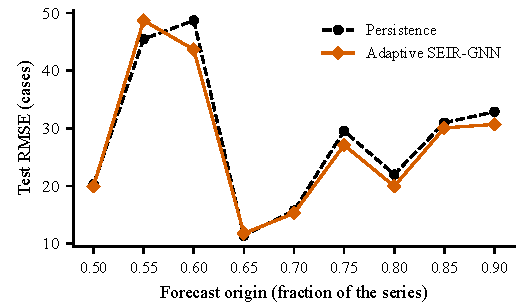
\includegraphics[width=\columnwidth]{figures/fig_origins.pdf}
\caption{Seed-averaged RMSE by forecast origin for persistence and the Adaptive SEIR-GNN.}
\label{fig:origins}
\end{figure}

\begin{figure}[t]
\centering
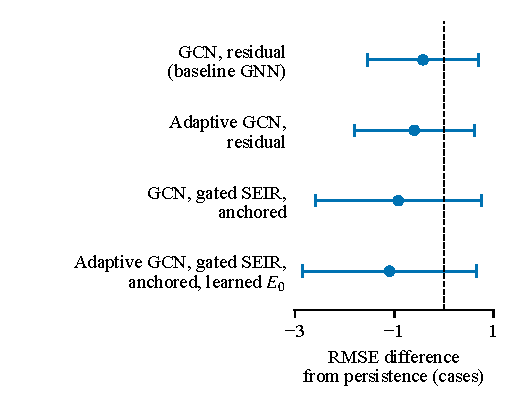
\includegraphics[width=\columnwidth]{figures/fig_forest.pdf}
\caption{Paired RMSE differences from persistence with descriptive 95\% $t$ intervals over nine seed-averaged origins. Negative values favour the model.}
\label{fig:forest}
\end{figure}

\begin{figure*}[t]
\centering
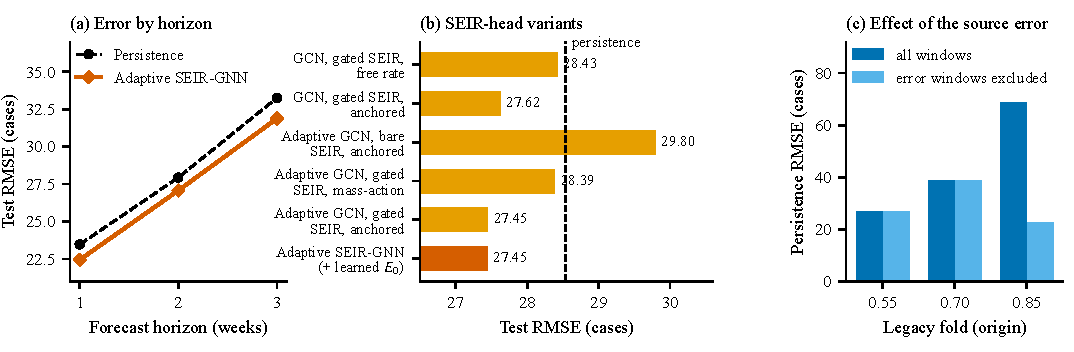
\includegraphics[width=\textwidth]{figures/fig_results.pdf}
\caption{(a) RMSE by forecast horizon. (b) SEIR-head ablations; the dashed line is persistence. (c) Persistence RMSE on the three legacy folds with all windows and after excluding the six windows that touch the erroneous source row. Panels (a) and (b) use the nine-origin development protocol.}
\label{fig:results}
\end{figure*}

\subsection{What the SEIR design contributes}
The clearest within-family result is the transmission-rate parameterization.
On the same GCN encoder, replacing the free gated SEIR rate (28.43 RMSE) with the population-and-susceptibility anchored rate lowers RMSE to 27.62 (Fig.~\ref{fig:results}b). % EV-210, EV-213
Gating is also important: the adaptive bare anchored SEIR head reaches 29.80, above persistence, whereas the corresponding gated anchored variant reaches 27.45. % EV-211, EV-214
The mass-action variant scores 28.39, and encoder-derived $E_0$ changes 27.45 only marginally. % EV-212, EV-214, EV-215
An adaptive graph encoder with a residual head and no SEIR simulator reaches 27.94. % EV-208
Because the nine-origin experiment does not include a matched adaptive gated non-SEIR head, these comparisons do not isolate the effect of the SEIR equations themselves; historical three-origin controls are mixed and are therefore kept supplementary.

\subsection{Forecast horizon and source-data quality}
The Adaptive SEIR-GNN is below persistence at each horizon by 1.03, 0.86, and 1.38 cases for weeks one, two, and three, respectively. % EV-153
Persistence RMSE rises from 23.47 at one week to 33.26 at three weeks; the GCN residual baseline rises from 23.24 to 32.47. % EV-225
On the legacy array, excluding the six windows that touch the erroneous report lowers mean persistence RMSE from 44.80 to 29.52 and the last legacy fold from 68.62 to 22.80 (Fig.~\ref{fig:results}c). % EV-220
The effect of this single data error is therefore far larger than the 1.10-case point-estimate gap between the best learned configuration and persistence. % EV-220, EV-215

\section{Discussion and Limitations}\label{sec:discussion}
The results support a narrower conclusion than ``SEIR improves forecasting.''
A graph encoder can be coupled to a daily SEIR decoder without losing short-horizon competitiveness, and an epidemiologically scaled transmission anchor substantially improves the gated SEIR head relative to its free-rate counterpart.
The full hybrid model has the lowest observed RMSE, but its approximately 3.8\% reduction relative to persistence is small compared with variation across forecast origins and is not statistically reliable under the present analysis.

The ablations also show why the mechanism should not be credited too broadly.
A bare anchored simulator is worse than persistence, while gating recovers much of the performance; a graph-only adaptive residual model is already competitive.
Thus the evidence supports the combined design---persistence anchoring, gating, graph representation, and SEIR constraints---but does not establish that the compartment equations alone add predictive information.
This distinction is important because weekly dengue counts are strongly persistent over a three-week horizon, leaving a complex model little room to improve unless it captures changes that recent counts do not.

The data audit is independently important.
One source-table formula error changes the legacy persistence benchmark by more than the entire gap among the strongest models.
This demonstrates that source verification can matter more than architectural refinement when benchmark series are assembled from public surveillance reports.

Several limitations prevent confirmatory claims.
The origin grid and some adaptive/anchored variants were chosen after earlier development results were available; the held-out blocks also share two target weeks with the immediately preceding validation windows.
The historical runs use a benchmark graph with two non-border directed entries, and all neural models share one training setting rather than an equal tuning budget.
The nine-origin protocol lacks a matched gated non-SEIR adaptive control and does not include seasonal-naive or classical autoregressive baselines.
Finally, the SEIR decoder uses fixed disease-duration assumptions, a learned scaling of a base reporting fraction, a Colombo-derived susceptible fraction for every district, and no explicit mosquito, serotype, or waning-immunity compartments.
These limitations mean the present paper should be read as a rigorous audit of development evidence, not as an untouched prospective validation.

A decisive next study is therefore straightforward: freeze the model family and analysis plan before opening a later time period, correct the graph, purge target overlap at partition boundaries, add matched gated non-SEIR and simple seasonal/autoregressive baselines, give compared neural models validation-only tuning budgets, and test sensitivity to the epidemiological parameters.
Such an untouched evaluation would answer whether the observed point-estimate advantage survives outside development data.

\section{Conclusion}
We presented an SEIR-informed graph forecaster for weekly district-level dengue in Sri Lanka and evaluated it against persistence on a reconstructed surveillance series.
The proposed configuration records the lowest observed RMSE, 27.45 versus 28.54 for persistence, while population-and-susceptibility anchoring improves the corresponding gated SEIR head within the same GCN encoder. % EV-200, EV-210, EV-213, EV-215
However, the nine-origin evidence does not establish a statistically reliable advantage, and the current ablations cannot attribute the point-estimate gain uniquely to the SEIR equations. % EV-219
The source-data audit is equally consequential: one spreadsheet error changes the legacy persistence benchmark far more than the best model's observed gain. % EV-220
The main lesson is therefore methodological as well as architectural: mechanistic graph forecasting is feasible and competitive, but claims of improvement should rest on source-checked data, strong simple baselines, matched ablations, and an untouched evaluation period.

\bibliographystyle{IEEEtran}
\bibliography{refs}
\end{document}
